\documentclass[a4paper,11pt]{article}
\usepackage[latin1]{inputenc}
\usepackage[T1]{fontenc}
\usepackage{bbm}
\usepackage{amsmath}
\usepackage{indentfirst}
\usepackage{fullpage}
\usepackage{url}
\usepackage{geometry}
\geometry{verbose,tmargin=3cm,bmargin=2cm,lmargin=2cm,rmargin=2cm}
\usepackage{graphicx}
\usepackage{epstopdf}
\usepackage[center,footnotesize]{caption}
\usepackage[section]{placeins}
\usepackage{subfig}
\DeclareRobustCommand{\greektext}{%
  \fontencoding{LGR}\selectfont\def\encodingdefault{LGR}}
\DeclareRobustCommand{\textgreek}[1]{\leavevmode{\greektext #1}}
\DeclareFontEncoding{LGR}{}{}
\DeclareTextSymbol{\~}{LGR}{126}
\title{Series 3}
\date{}
\author{Genomics and bioinformatics - Week 4 - October 9, 2011}
\begin{document}
\maketitle


\section{Sequence alignment: Needleman-Wunsch}
In this exercise you will manually perform a global alignment of two sequences using the
Needleman-Wunsch algorithm and based on the following scoring scheme: for $X,Y$ in $\{A,T,G,C,-\}$, 
$$
M(X,Y) = \left\{ 
\begin{array}{l}
	+1 \quad\text{if}\quad X = Y \\
	-2 \quad\text{if}\quad X = - \quad\text{or}\quad Y = - \\
	-1 \quad \text{otherwise}
\end{array} \right.
$$
Sequence 1: \texttt{GAATTCAG}\\
Sequence 2: \texttt{GGATCG}.
\vspace{0.5cm}
\begin{center}

\includegraphics[width=0.8\textwidth]{matrix.png}
\end{center}
\vspace{0.5cm}

The best alignment is: ........\\

\newpage 

\section{Pair Hidden Markov Model}

In this exercise, we will construct a pair Hidden Markov Model for
the same sequences as in the first exercise and align them using the
path with maximum probability. The maximum probability path and the 
corresponding alignment are calculated by an algorithm called the Viterbi Algorithm. 
You will see through the exercise that the Viterbi algorithm is actually equivalent
to the Needleman-Wunsch algorithm.


\begin{figure}[h]
\begin{center}
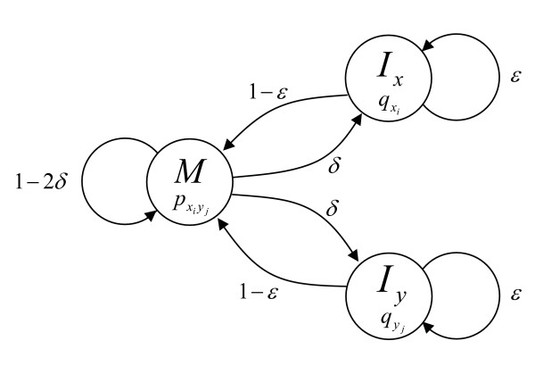
\includegraphics[width=0.5\textwidth]{HMM.jpg}
\caption{Pair Hidden Markov Model}
\label{fig:HMM}
\end{center}
\end{figure}


The Pair HMM consists of the following parameters (see fig.~\ref{fig:HMM}):

\begin{itemize}
\item Three states:

State M matches one letter from each sequence.

State D (Deletion) inserts a gap to the second sequence.

State I (Insertion) inserts a gap to the first sequence.

\item Emission probabilities:

$p(x,y) =$ probability of emitting a pair of characters $[x,y]$ in state M ($x,y \in \{A,T,G,C\}$).

$p(x) = p(x,-) =$ probability of emitting a pair of characters $[x,-]$ in state D.

$p(y) = p(-,y) =$ probability of emitting a pair of characters $[-,y]$ in state I.

\item Transition probabilities (affine gaps case):

$\delta$ = probability of opening a gap

$\varepsilon$ = probability of extending a gap
\end{itemize}

To make correspondence to the Needleman-Wunsch algorithm with the scores given in Exercise 1,


$$S(x,y)=log_2\frac{p(x,y)}{p(x)\; p(y)} \quad , \quad d=log_2(\delta) \quad ,$$

S(x,y) = 1 if $x=y$, 

S(x,y) = -1 if $x\neq y$,

d = e = -2 for (linear) gap penalty.

\newpage
The Viterbi algorithm goes through the three steps:\\


Step 1: Initialization:\\

$V_M(0,0):=0$

$V_D(0,0):=-\infty$

$V_I(0,0):=-\infty$

$V_*(-1,j)=V_*(i,-1):=-\infty \;$ ($_*$ accounts for either M, D or I)
\vspace{0.5cm}

Step 2: Recursion:
\begin{eqnarray}
&&
V_M(i,j) =S(x_{i},y_{j})+\max 
	\left\{ \begin{array}{l}
	 V_M(i-1,j-1) \\
     V_D(i-1,j-1) \\
     V_I(i-1,j-1)
    \end{array} \right.\nonumber\\
&&
V_D(i,j) =\max \left\{ 
    \begin{array}{ll}
     V_M(i-1,j)-d \\
     V_D(i-1,j)-e 
    \end{array} \right.\nonumber\\
&&
V_I(i,j) =\max \left\{ 
    \begin{array}{ll}
     V_M(i,j-1)-d\\
     V_I(i,j-1)-e
    \end{array} \right.\nonumber
\end{eqnarray}


Step 3: Termination:

$$V_E(n,m)=\max(V_M(n,m),V_D(n,m),V_I(n,m)) \qquad \forall m,n$$

\underline{Questions:}
\begin{enumerate}
\item Deduce the emission probability matrix and the transition probabilities of the HMM.\\
	\textit{Note}: suppose that independent emissions of A,T,G,C are equiprobable (1/4).
\item Use the algorithm shown above to generate $V_M, V_D, V_I, V_E$.
\item Deduce the alignment based on these matrices.
\end{enumerate}

\newpage

Matrix $V_M$:
\begin{center}

\includegraphics[width=0.8\textwidth]{matrix.png}
\end{center}
\vspace{1.5cm}

Matrix $V_D$:
\begin{center}

\includegraphics[width=0.8\textwidth]{matrix.png}
\end{center}
\vspace{1.5cm}

\newpage 

Matrix $V_I$: 
\begin{center}

\includegraphics[width=0.8\textwidth]{matrix.png}
\end{center}
\vspace{0.5cm}

Backtracking matrix $V_E$:
\begin{center}

\includegraphics[width=0.8\textwidth]{matrix.png}
\end{center}
\vspace{0.5cm}

The possible alignments are: ........................


\end{document}
